\documentclass{article}
\usepackage[utf8]{inputenc}
\usepackage[papersize={8.5in,11in},margin=0.8in]{geometry}
\usepackage{xcolor}
\usepackage{color, colortbl}
\usepackage{graphicx}
\usepackage{tikz}
\usepackage{amssymb}
\usetikzlibrary{positioning}


\title{MATH 505 Assignment 7}
\author{John Caruthers}
\date\today

\begin{document}
\maketitle

\begin{itemize}
    \item[1.] If possible, find a route for the Salesman(Euler Path) in the system.  Find a route for the Inspector (Hamilton Path)
    
    \begin{center}
        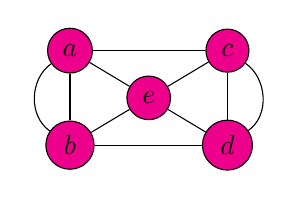
\begin{tikzpicture}
           [dot/.style = {draw,fill=magenta,circle}]
            \node[dot] (a) at (0, -0.5) {$a$};
            \node[dot] (b) at (0,-1.7) {$b$};
            \node[dot] (c) at (2, -0.5) {$c$};
            \node[dot] (d) at (2, -1.7) {$d$};
            \node[dot] (e) at (1,-1.1) {$e$};
        
            \path[-] (a) edge (b);
            \path[-] (b) edge (e);
            \path[-] (e) edge (c);
            \path[-] (a) edge[out=215,in=145] (b);
            \path[-] (c) edge[out=325,in=35] (d);
            \path[-] (a) edge (c);
            \path[-] (b) edge (d);
            \path[-] (a) edge (e);
            \path[-] (e) edge (d);
            \path[-] (c) edge (d);
            
            \end{tikzpicture}
    \end{center}
    
    {\color{blue}
    Inspector route: $a,b$(curved)$,a$(straight)$,e,b,d,e,c,d$(straight)$,c$(curved)$,a$\\
    Salesman route: $a,b$(straight)$,e,d,c$(straight)}
    
    \item[2.]If possible, find a route for the Salesman in this system. Find a route for the Inspector.
    
    \begin{center}
        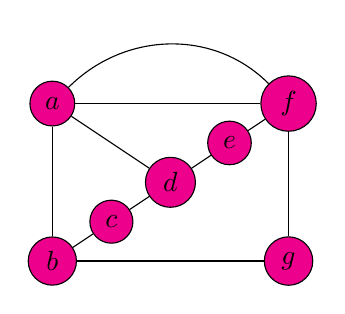
\begin{tikzpicture}
           [dot/.style = {draw,fill=magenta,circle}]
            \node[dot] (a) at (0, -0.5) {$a$};
            \node[dot] (b) at (0,-2.5) {$b$};
            \node[dot] (c) at (0.75,-2) {$c$};
            \node[dot] (d) at (1.5,-1.5) {$d$};
            \node[dot] (e) at (2.25, -1) {$e$};
            \node[dot] (f) at (3, -0.5) {$f$};
            \node[dot] (g) at (3, -2.5) {$g$};
        
            \path[-] (a) edge (b);
            \path[-] (b) edge (c);
            \path[-] (c) edge (d);
            \path[-] (d) edge (e);
            \path[-] (e) edge (f);
            \path[-] (a) edge[out=45,in=135] (f);
            \path[-] (a) edge (f);
            \path[-] (a) edge (d);
            \path[-] (b) edge (g);
            \path[-] (f) edge (g);
            
            \end{tikzpicture}
    \end{center}
    
    {\color{blue}
    Inspector route: $d,a,f$(straight)$,a$(curved)$,b,g,f,e,d,c,b$\\
    Salesman route: $a,b,g,f,e,d,c$}
    
    \item[3.] Complete the table for the following road maps.
    
    \begin{center}
\begin{tabular}{|c|c|c|c|}
    \hline
    Map & Number Odd Nodes & Number Even Nodes & Euler Path\\
    \hline
    $a$ & 4 & 3 & $no$\\
    \hline
    $b$ & 2 & 4 & $yes$\\
    \hline
    $c$ & 2 & 4 & $yes$\\
    \hline
    $d$ & 8 & 4 & $no$\\
    \hline
    $e$ & 4 & 1 & $no$\\
    \hline
    $f$ & 0 & 8 & $yes$\\
    \hline
\end{tabular}
    \end{center}
\end{itemize}

\end{document}
